% Options for packages loaded elsewhere
\PassOptionsToPackage{unicode}{hyperref}
\PassOptionsToPackage{hyphens}{url}
%
\documentclass[
]{article}
\usepackage{amsmath,amssymb}
\usepackage{iftex}
\ifPDFTeX
  \usepackage[T1]{fontenc}
  \usepackage[utf8]{inputenc}
  \usepackage{textcomp} % provide euro and other symbols
\else % if luatex or xetex
  \usepackage{unicode-math} % this also loads fontspec
  \defaultfontfeatures{Scale=MatchLowercase}
  \defaultfontfeatures[\rmfamily]{Ligatures=TeX,Scale=1}
\fi
\usepackage{lmodern}
\ifPDFTeX\else
  % xetex/luatex font selection
\fi
% Use upquote if available, for straight quotes in verbatim environments
\IfFileExists{upquote.sty}{\usepackage{upquote}}{}
\IfFileExists{microtype.sty}{% use microtype if available
  \usepackage[]{microtype}
  \UseMicrotypeSet[protrusion]{basicmath} % disable protrusion for tt fonts
}{}
\makeatletter
\@ifundefined{KOMAClassName}{% if non-KOMA class
  \IfFileExists{parskip.sty}{%
    \usepackage{parskip}
  }{% else
    \setlength{\parindent}{0pt}
    \setlength{\parskip}{6pt plus 2pt minus 1pt}}
}{% if KOMA class
  \KOMAoptions{parskip=half}}
\makeatother
\usepackage{xcolor}
\usepackage[margin=1in]{geometry}
\usepackage{graphicx}
\makeatletter
\def\maxwidth{\ifdim\Gin@nat@width>\linewidth\linewidth\else\Gin@nat@width\fi}
\def\maxheight{\ifdim\Gin@nat@height>\textheight\textheight\else\Gin@nat@height\fi}
\makeatother
% Scale images if necessary, so that they will not overflow the page
% margins by default, and it is still possible to overwrite the defaults
% using explicit options in \includegraphics[width, height, ...]{}
\setkeys{Gin}{width=\maxwidth,height=\maxheight,keepaspectratio}
% Set default figure placement to htbp
\makeatletter
\def\fps@figure{htbp}
\makeatother
\setlength{\emergencystretch}{3em} % prevent overfull lines
\providecommand{\tightlist}{%
  \setlength{\itemsep}{0pt}\setlength{\parskip}{0pt}}
\setcounter{secnumdepth}{-\maxdimen} % remove section numbering
\ifLuaTeX
  \usepackage{selnolig}  % disable illegal ligatures
\fi
\usepackage{bookmark}
\IfFileExists{xurl.sty}{\usepackage{xurl}}{} % add URL line breaks if available
\urlstyle{same}
\hypersetup{
  pdftitle={Taller de Github y code control},
  hidelinks,
  pdfcreator={LaTeX via pandoc}}

\title{Taller de Github y code control}
\author{}
\date{\vspace{-2.5em}}

\begin{document}
\maketitle

\subsection{Taller de github - Laboratorio de Interacciones Ecológicas y
Conservación:}\label{taller-de-github---laboratorio-de-interacciones-ecoluxf3gicas-y-conservaciuxf3n}

\subsection{\texorpdfstring{\textbf{Entonces, ¿Que es Git y
Github?}}{Entonces, ¿Que es Git y Github?}}\label{entonces-que-es-git-y-github}

\subsubsection{\texorpdfstring{\textbf{Github}: Es una plataforma en la
nube que aloja repositorios de còdigo (públicos o privados), imágenes,
certficados e inclusos cvs. Pero lo mas interesante es que permitie que
varias personas trabajen en un mismo proyecto, creando código para un
paper por ejemplo, de forma
ordenada.}{Github: Es una plataforma en la nube que aloja repositorios de còdigo (públicos o privados), imágenes, certficados e inclusos cvs. Pero lo mas interesante es que permitie que varias personas trabajen en un mismo proyecto, creando código para un paper por ejemplo, de forma ordenada.}}\label{github-es-una-plataforma-en-la-nube-que-aloja-repositorios-de-cuxf2digo-puxfablicos-o-privados-imuxe1genes-certficados-e-inclusos-cvs.-pero-lo-mas-interesante-es-que-permitie-que-varias-personas-trabajen-en-un-mismo-proyecto-creando-cuxf3digo-para-un-paper-por-ejemplo-de-forma-ordenada.}

\subsubsection{\texorpdfstring{\url{https://github.com/ibartomeus}}{https://github.com/ibartomeus}}\label{httpsgithub.comibartomeus}

\subsubsection{\texorpdfstring{\url{https://github.com/weecology}}{https://github.com/weecology}}\label{httpsgithub.comweecology}

\subsubsection{\texorpdfstring{\url{https://github.com/RadicalCommEcol}}{https://github.com/RadicalCommEcol}}\label{httpsgithub.comradicalcommecol}

\subsubsection{\texorpdfstring{\url{https://github.com/VicMarquez}}{https://github.com/VicMarquez}}\label{httpsgithub.comvicmarquez}

\subsubsection{\texorpdfstring{\textbf{Git}: Es un sistema que permite
rastrear cambios en archivos de código, facilitando la colaboración y la
recuperación de versiones anteriores. Github sirve de interfaz para
visualizar y alamacenar estos
cambios.}{Git: Es un sistema que permite rastrear cambios en archivos de código, facilitando la colaboración y la recuperación de versiones anteriores. Github sirve de interfaz para visualizar y alamacenar estos cambios.}}\label{git-es-un-sistema-que-permite-rastrear-cambios-en-archivos-de-cuxf3digo-facilitando-la-colaboraciuxf3n-y-la-recuperaciuxf3n-de-versiones-anteriores.-github-sirve-de-interfaz-para-visualizar-y-alamacenar-estos-cambios.}

\newpage

\subsubsection{El repositorio en Github es básicamente una carpeta que
contiene todos los archivos de tu proyecto (código, base de datos,
readme, etc) y el historial de revisiones de cada archivo. Aquí es donde
guardaremos todos los archivos del proyecto (¡cuidado con el
tamaño!)}\label{el-repositorio-en-github-es-buxe1sicamente-una-carpeta-que-contiene-todos-los-archivos-de-tu-proyecto-cuxf3digo-base-de-datos-readme-etc-y-el-historial-de-revisiones-de-cada-archivo.-aquuxed-es-donde-guardaremos-todos-los-archivos-del-proyecto-cuidado-con-el-tamauxf1o}

\subsubsection{Los repositorios pueden ser públicos o privados, y su
propiedad puede ser compartida con sus
colaboradores.}\label{los-repositorios-pueden-ser-puxfablicos-o-privados-y-su-propiedad-puede-ser-compartida-con-sus-colaboradores.}

\subsubsection{Git es una de las herramientas fundamentales para la
colaboración y el trabajo en equipo. Mantenemos un seguimiento de todos
los cambios en los archivos, con explicaciones sobre quién y por qué
realizó esos
cambios.}\label{git-es-una-de-las-herramientas-fundamentales-para-la-colaboraciuxf3n-y-el-trabajo-en-equipo.-mantenemos-un-seguimiento-de-todos-los-cambios-en-los-archivos-con-explicaciones-sobre-quiuxe9n-y-por-quuxe9-realizuxf3-esos-cambios.}

\subsubsection{Al trabajar con GitHub, siempre tenemos una carpeta local
y una carpeta remota. Hacemos los cambios localmente, los enviamos (push
o pusheo) al control remoto y extraemos (pull) los cambios realizados
por
otros}\label{al-trabajar-con-github-siempre-tenemos-una-carpeta-local-y-una-carpeta-remota.-hacemos-los-cambios-localmente-los-enviamos-push-o-pusheo-al-control-remoto-y-extraemos-pull-los-cambios-realizados-por-otros}

\newpage

\section{Main commands}\label{main-commands}

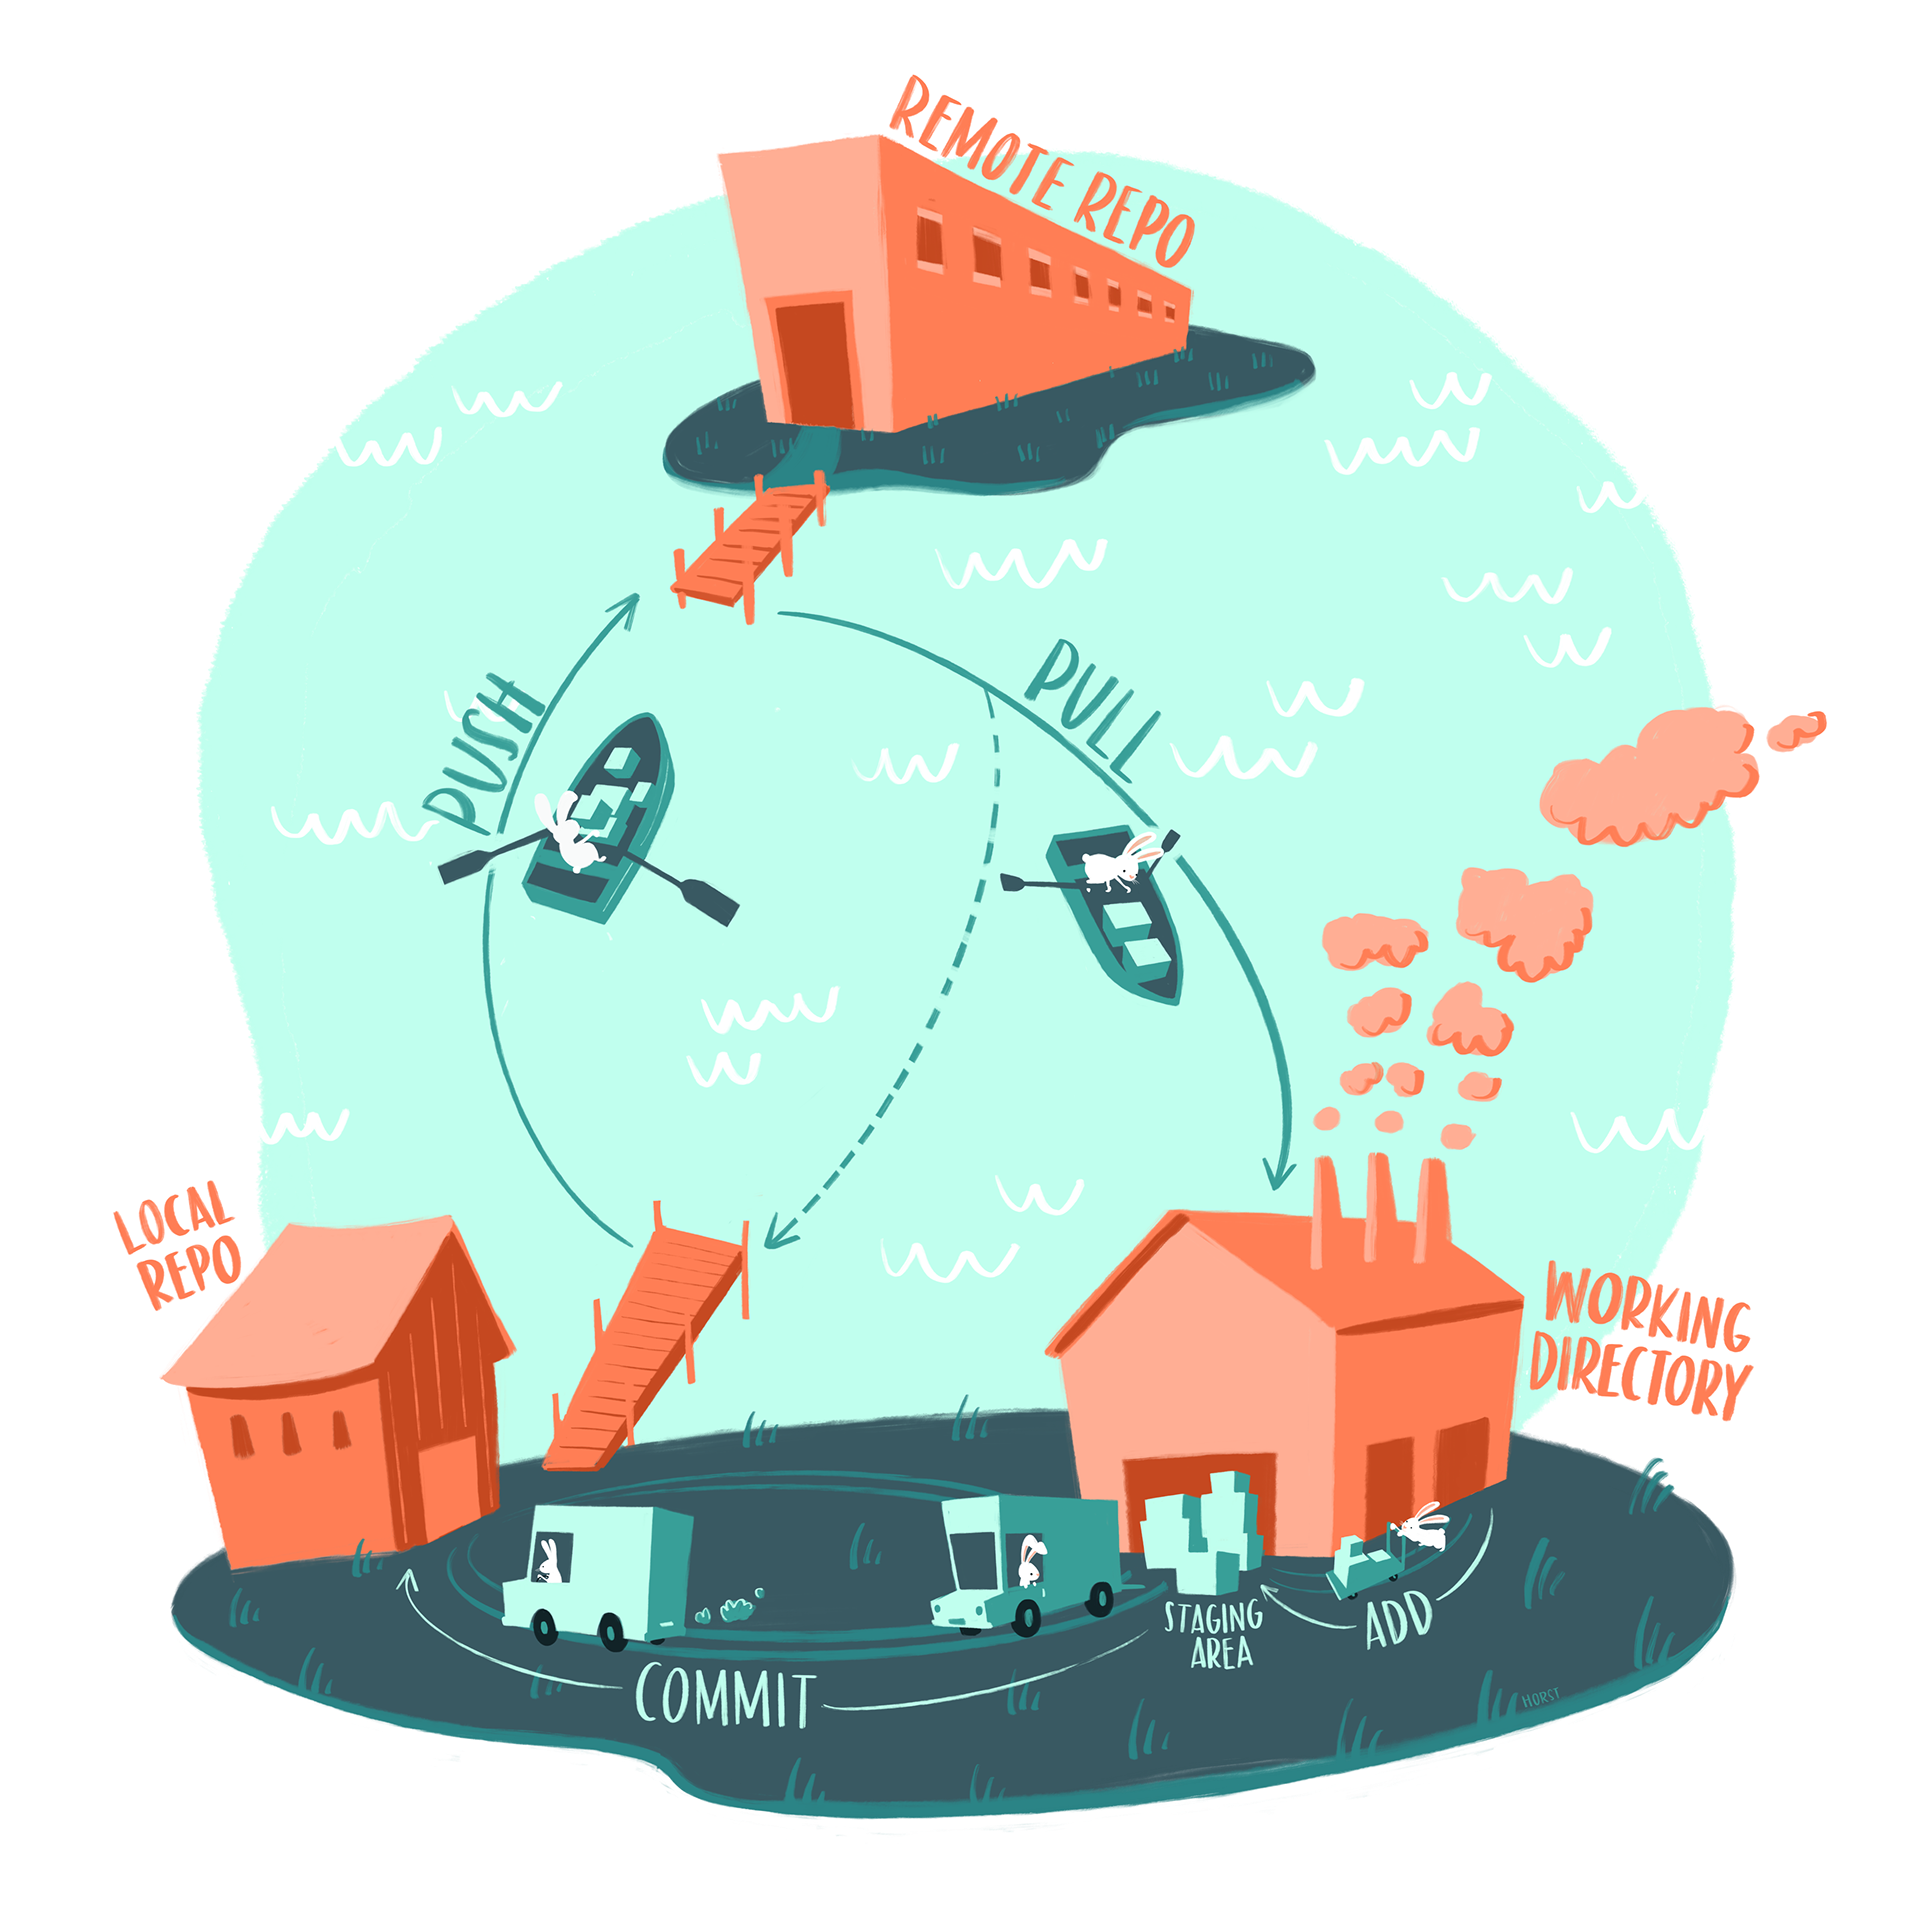
\includegraphics{git_workflow.png} \#\#\# \textbf{git clone}: Clone
(download) a repository that already exists on GitHub, including all of
the files, branches, and commits.

\subsubsection{\texorpdfstring{\textbf{git pull}: It synchronizes the
local development repository with updates from the corresponding remote
repository on GitHub. In other words, it fetches and incorporates the
modifications made by our team into our local
repository.}{git pull: It synchronizes the local development repository with updates from the corresponding remote repository on GitHub. In other words, it fetches and incorporates the modifications made by our team into our local repository.}}\label{git-pull-it-synchronizes-the-local-development-repository-with-updates-from-the-corresponding-remote-repository-on-github.-in-other-words-it-fetches-and-incorporates-the-modifications-made-by-our-team-into-our-local-repository.}

\subsubsection{\texorpdfstring{\textbf{git status}: This command
displays our current status, including the state of local changes, the
branch we are on, and any other relevant
information.}{git status: This command displays our current status, including the state of local changes, the branch we are on, and any other relevant information.}}\label{git-status-this-command-displays-our-current-status-including-the-state-of-local-changes-the-branch-we-are-on-and-any-other-relevant-information.}

\subsubsection{\texorpdfstring{\textbf{git add + git commit + git push}:
These commands will enable us to upload our local changes to the
repository.}{git add + git commit + git push: These commands will enable us to upload our local changes to the repository.}}\label{git-add-git-commit-git-push-these-commands-will-enable-us-to-upload-our-local-changes-to-the-repository.}

\subsubsection{\texorpdfstring{\textbf{git add}: This is the initial
step where we add new or modified files in the local working directory
to the Git staging area. This process prepares the files to be included
in the next
commit.}{git add: This is the initial step where we add new or modified files in the local working directory to the Git staging area. This process prepares the files to be included in the next commit.}}\label{git-add-this-is-the-initial-step-where-we-add-new-or-modified-files-in-the-local-working-directory-to-the-git-staging-area.-this-process-prepares-the-files-to-be-included-in-the-next-commit.}

\subsubsection{\texorpdfstring{\textbf{git commit -m''a descriptive
message''}: This command records our changes in the version history.
Anything that has been staged using git add will be permanently stored
in the history. Additionally, when using this command, we can include a
descriptive message that explains the nature of the changes we
made.}{git commit -m''a descriptive message'': This command records our changes in the version history. Anything that has been staged using git add will be permanently stored in the history. Additionally, when using this command, we can include a descriptive message that explains the nature of the changes we made.}}\label{git-commit--ma-descriptive-message-this-command-records-our-changes-in-the-version-history.-anything-that-has-been-staged-using-git-add-will-be-permanently-stored-in-the-history.-additionally-when-using-this-command-we-can-include-a-descriptive-message-that-explains-the-nature-of-the-changes-we-made.}

\subsubsection{\texorpdfstring{\textbf{git push}: Uploads all local
commits to the remote
repository.}{git push: Uploads all local commits to the remote repository.}}\label{git-push-uploads-all-local-commits-to-the-remote-repository.}

\newpage

\subsubsection{\texorpdfstring{Para poder utilizar GitHub, el primer
paso será crear y configurar nuestra cuenta
(\url{https://docs.github.com/en/get-started/onboarding/getting-started-with-your-github-account})
Por lo tanto, necesitamos crear una cuenta en GitHub y verificar nuestro
correo
electrónico.}{Para poder utilizar GitHub, el primer paso será crear y configurar nuestra cuenta (https://docs.github.com/en/get-started/onboarding/getting-started-with-your-github-account) Por lo tanto, necesitamos crear una cuenta en GitHub y verificar nuestro correo electrónico.}}\label{para-poder-utilizar-github-el-primer-paso-seruxe1-crear-y-configurar-nuestra-cuenta-httpsdocs.github.comenget-startedonboardinggetting-started-with-your-github-account-por-lo-tanto-necesitamos-crear-una-cuenta-en-github-y-verificar-nuestro-correo-electruxf3nico.}

\subsubsection{\texorpdfstring{El siguiente paso es instalar Git.
También necesitaremos crear un token de acceso personal (esta es la
parte mas difícil), el último paso para autenticar nuestra identidad al
interactuar con GitHub desde un dispositivo local. La primera vez que
intentemos interactuar con un repositorio remoto de GitHub desde nuestro
dispositivo, GitHub nos pedirá nuestro nombre de usuario y nuestro token
(\url{https://docs.github.com/en/authentication/keeping-your-account-and-data-secure/managing-your-personal-access-tokens}).}{El siguiente paso es instalar Git. También necesitaremos crear un token de acceso personal (esta es la parte mas difícil), el último paso para autenticar nuestra identidad al interactuar con GitHub desde un dispositivo local. La primera vez que intentemos interactuar con un repositorio remoto de GitHub desde nuestro dispositivo, GitHub nos pedirá nuestro nombre de usuario y nuestro token (https://docs.github.com/en/authentication/keeping-your-account-and-data-secure/managing-your-personal-access-tokens).}}\label{el-siguiente-paso-es-instalar-git.-tambiuxe9n-necesitaremos-crear-un-token-de-acceso-personal-esta-es-la-parte-mas-difuxedcil-el-uxfaltimo-paso-para-autenticar-nuestra-identidad-al-interactuar-con-github-desde-un-dispositivo-local.-la-primera-vez-que-intentemos-interactuar-con-un-repositorio-remoto-de-github-desde-nuestro-dispositivo-github-nos-pediruxe1-nuestro-nombre-de-usuario-y-nuestro-token-httpsdocs.github.comenauthenticationkeeping-your-account-and-data-securemanaging-your-personal-access-tokens.}

\subsection{Como generar un clave ssh:}\label{como-generar-un-clave-ssh}

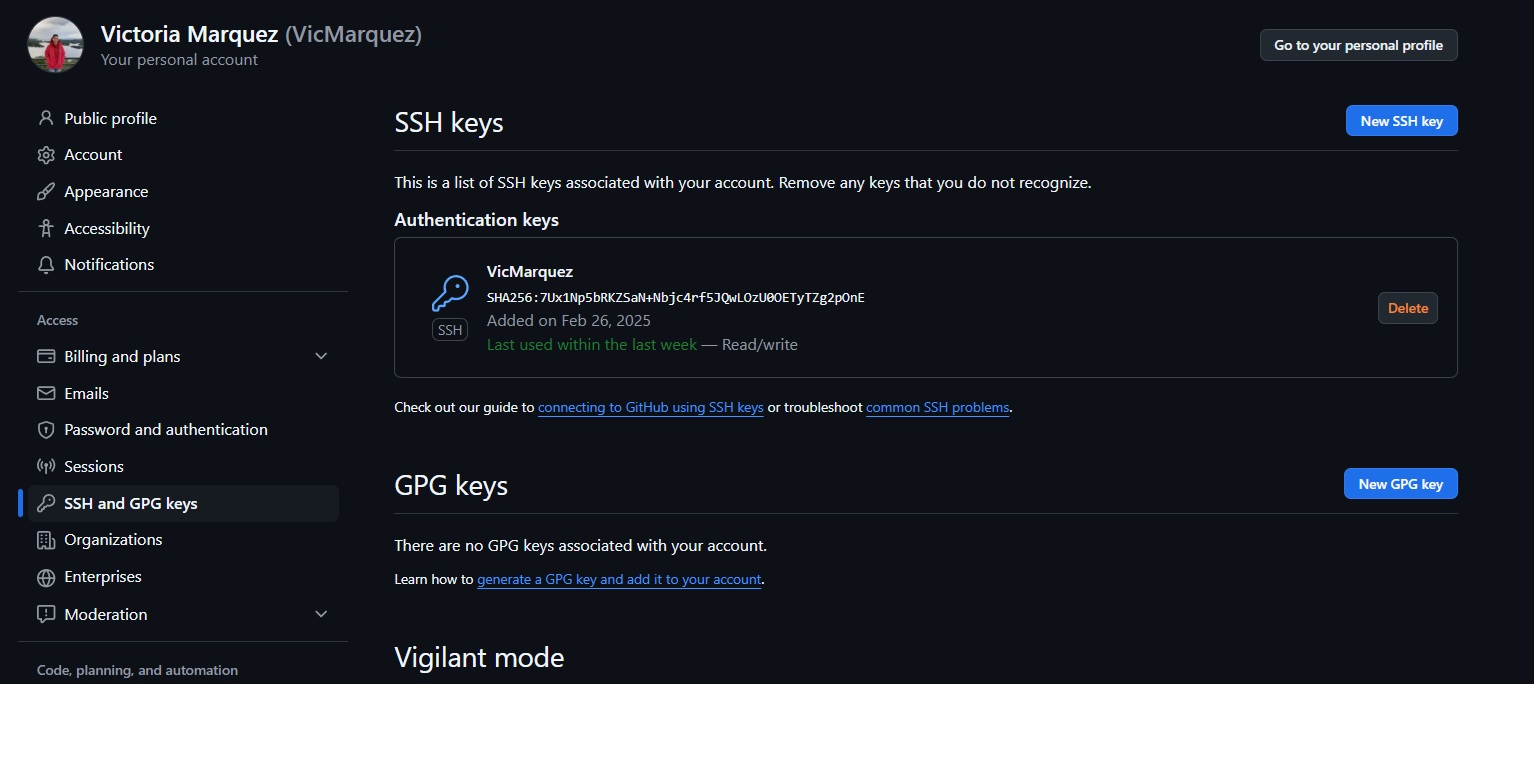
\includegraphics{key.jpg}

\texttt{ssh-keygen\ -t\ ed25519\ -C\ "tu-email@ejemplo.com"}

\texttt{ssh-keygen\ -t\ rsa\ -b\ 4096\ -C\ "tu-email@ejemplo.com"}

\subsubsection{Te pedirá elegir una ubicación para guardar la clave.
Presioná Enter para aceptar la ubicación por defecto
(\textasciitilde/.ssh/id\_ed25519). Cuando pregunte por una contraseña
opcional, podés dejarla vacía o escribir una si querés más
seguridad.}\label{te-pediruxe1-elegir-una-ubicaciuxf3n-para-guardar-la-clave.-presionuxe1-enter-para-aceptar-la-ubicaciuxf3n-por-defecto-.sshid_ed25519.-cuando-pregunte-por-una-contraseuxf1a-opcional-poduxe9s-dejarla-vacuxeda-o-escribir-una-si-queruxe9s-muxe1s-seguridad.}

\subsubsection{Agregar a Github}\label{agregar-a-github}

\subsubsection{Settings: SSH and GPG
keys}\label{settings-ssh-and-gpg-keys}

\subsubsection{Clic en New SSH key.}\label{clic-en-new-ssh-key.}

\subsubsection{Poner un nombre descriptivo (por ejemplo, ``Mi PC
RStudio'').}\label{poner-un-nombre-descriptivo-por-ejemplo-mi-pc-rstudio.}

\subsubsection{Pegar la clave copiada en el campo ``Key'' y hacé clic en
Add SSH
key.}\label{pegar-la-clave-copiada-en-el-campo-key-y-hacuxe9-clic-en-add-ssh-key.}

\end{document}
